Analisaremos dois casos: os com enrolamento fechado e aqueles com enrolamento aberto.

\subsection{Enrolamento fechado}

Os enrolamentos fechados para induzidos rotativos de alternadores podem ser de anel ou de tambor, dos mesmos tipos usados em corrente contínua. A diferença entre os enrolamentos destinados à corrente alternada e os destinados à corrente contínua consiste no fato de que os primeiros utilizam dois anéis coletores e os segundos usarem comutadores de lâminas.

\begin{figure}[ht!]
\center 
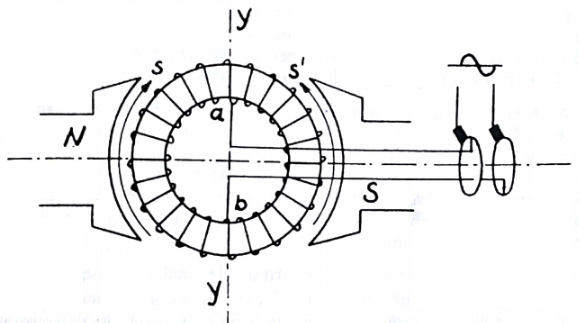
\includegraphics[scale=0.6]{imagens/5.png}
\caption{Enrolamento de anel bipolar.}
\end{figure}

A diferença de potencial entre os anéis tem valor máximo quando os terminais $a$ e $b$ passam pelo plano de inversão magnética YY (quando sai da porção positiva para a negativa da onda senoidal), pois neste caso, todos os condutores de cada via interna estão embaixo de um polo e suas f.e.m são concordes, conforme as setas $s$ e $s'$.

Estes enrolamentos são chamados de "fechados" pelo fato de se iniciar e terminar o enrolamento no mesmo ponto. Assim feito, o enrolamento é constituído por um circuito totalmente fechado, do qual são derivadas as ligações com o comutador ou os anéis coletores, conforme se tratar de corrente contínua ou corrente alternada.

\subsection{Enrolamento aberto}

Este tipo de enrolamento executa-se dispondo-se em série, nos canais periféricos do induzido, determinado número de bobinas. A distribuição de bobinas deve ser feito de forma a manter o equilíbrio do induzido. Cada bobina apresenta um lado embaixo de um polo Norte e outro sob o polo Sul.

\begin{figure}[ht!]
\center 
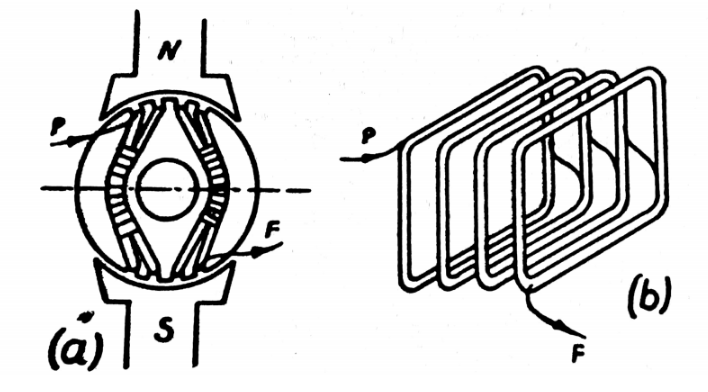
\includegraphics[scale=0.5]{imagens/6.PNG}
\caption{Enrolamento bipolar com quatro bobinas em série.}
\end{figure}

Os terminais do conjunto $P$ e $F$ são chamados arbitrariamente de princípio e fim do enrolamento e são ligados aos dois anéis coletores.

